
% This LaTeX was auto-generated from MATLAB code.
% To make changes, update the MATLAB code and republish this document.

\documentclass{article}
\usepackage{graphicx}
\usepackage{color}

\sloppy
\definecolor{lightgray}{gray}{0.5}
\setlength{\parindent}{0pt}

\begin{document}

    
    \begin{verbatim}
% This program generates the mandelbrot set

%Define the functions and fixed points.
phi = @(z,c) z^2 + c;
fixpt1 = @(c) (1 + sqrt(1-4*c))/2;
fixpt2 = @(c) (1 - sqrt(1-4*c))/2;
z0=0;       %madelbrot uses z0=0;
colormap jet;

M= ones(401,401);
for j=1:401                  % Try initial values with imaginary parts between
  y = -2+ (j-1)*.01;        %   -2 and 2
  for i=1:401                % and with real parts between
    x = -2 + (i-1)*.01;     %   -2 and 2.
    c = x + 1i*y;


    iflag1 = 0;     % iflag1 and iflag2 count the number of iterations
    iflag2 = 0;     %   when a root is within 1.e-6 of a fixed point;
    kcount = 0;      % kount is the total number of iterations.
    zk=z0;
    %compute the orb(0) for this particular c value
    while kcount < 1000 && abs(zk) < 100 && iflag1 < 10 && iflag2 < 10
      kcount = kcount+1;
      zk = phi(zk,c);           % This is the fixed point iteration.

      err1 = abs(zk-fixpt1(c));  % Test for convergence to fixpt1.
      if err1 < 1.e-6
         iflag1 = iflag1 + 1;
      else
         iflag1 = 0;
      end

      err2 = abs(zk-fixpt2(c));  % Test for convergence to fixpt2.
      if err2 < 1.e-6
        iflag2 = iflag2 + 1;
      else
        iflag2 = 0;
      end

    end

    if abs(zk)>100 %if the orbit diverged, fill in the color map
        M(j,i)=kcount; %the color for terms that diverged with similar
                        %kcounts will have similar color
    end
  end
end

image([-2 2],[-2 2],M),  % This plots the results.
pbaspect([1 1 1]); %keeps the x/y ratio even
axis xy % prevents inverted xy axis
\end{verbatim}

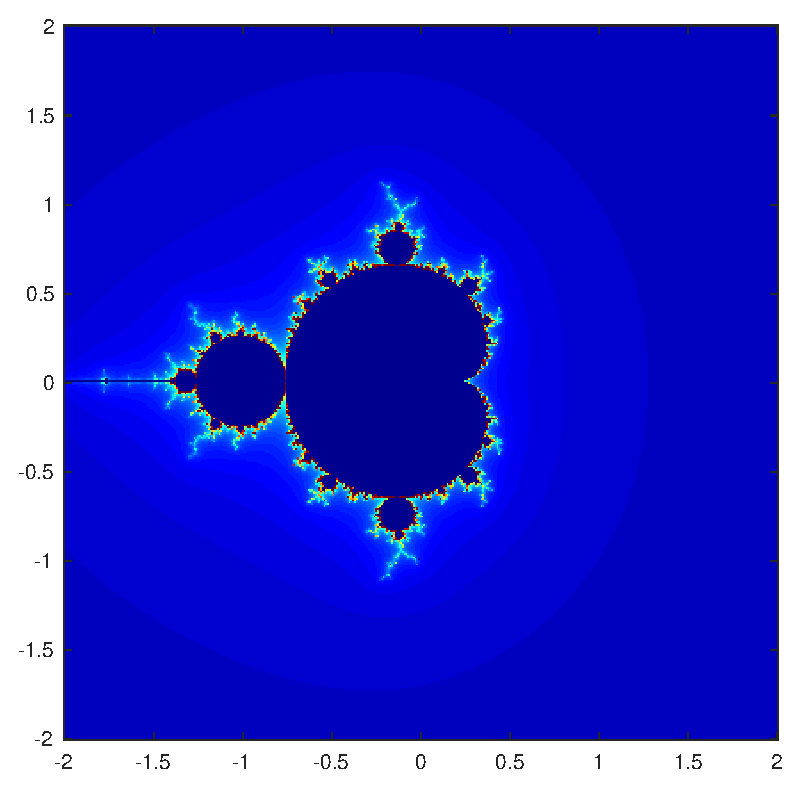
\includegraphics [width=4in]{Mandelbrot_01.eps}



\end{document}
    
